\documentclass{article}
\usepackage[T2A]{fontenc} %кирилица
\usepackage[utf8]{inputenc} %UTF-8
\usepackage[russian, english]{babel} %русский язык
\usepackage{graphicx} %картинки
\usepackage{float} %плавающие картинки
\usepackage[margin=20mm]{geometry} %настройка размеров
\usepackage{multicol} %колонны
\usepackage{enumerate} %списки
\usepackage{enumitem} %кастомизация списков
\usepackage{hyperref}
\usepackage{biblatex}

\linespread{0.87}
\setcounter{page}{282}
\setlength{\columnsep}{6mm}%distance between columns
\graphicspath{ {images/} }%defoult path to img
\renewcommand{\thefigure}{\arabic{figure}}
\setcounter{figure}{3}

\title{lab1}
\author{Zahar Matsukevich}
\date{September 2024}

\begin{document}
\fontsize{10}{14}\selectfont
\begin{multicols*}{2}

\par The principal component method consists of calculating 
eigenvectors and eigenvalues of the covariance matrix of 
the data space, then constructing projections in such a way 
that the direction of the maximum dispersion of the projection 
always coincides with the eigenvector having the maximum 
eigenvalue equal to the value of this dispersion. The 
covariance matrix after PCA processing can be seen in Figure \ref{figure4}. 

\begin{figure}[H]
    \centering
    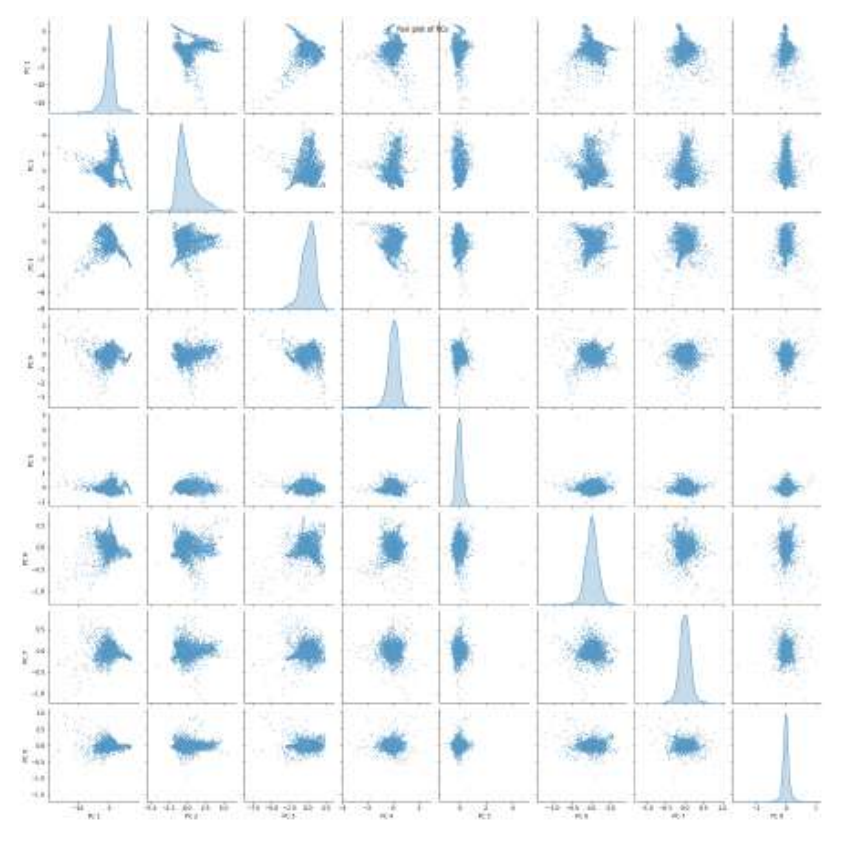
\includegraphics[width=\linewidth]{img4}
    \caption{\small \centering Visualization of the image covariance matrix with 8
    spectral bands. \label{figure4}}
\end{figure}

\par The next step of the algorithm is to reduce the dimension
of the data space, but in the case of multispectral
images this is not a necessary step: each projection
is a new image layer that stores the necessary data.
Instead, in [9] it is proposed to work only with the most
informative image from the resulting projections. 
\par Different images of the same class will have almost
identical spectral data ratios. Indeed, for Forest class
images the frequencies of 560 nm will prevail. and 842
nm., when for the SeaLake class 490 nm. and 945 nm.
As a consequence, since each cell of the covariance
matrix denotes either the variance of some layer of the
multispectral image if that cell lies on the diagonal, or
the covariance of two specific layers if it does not lie on
the diagonal, the covariance matrices for each class will
have the same patterns of dominant relationships. 

\begin{center}
    \uppercase\expandafter{\romannumeral 5}. Construction of a semantic form of the area 
\end{center}

\par If we consider the matrix as a vector, then using
the Word2vec technology from [10], from the previous
statements we can conclude that the image is converted
into a word that has metric characteristics, as shown in
Figure \ref{figure5}. 

\begin{figure}[H]
    \centering
    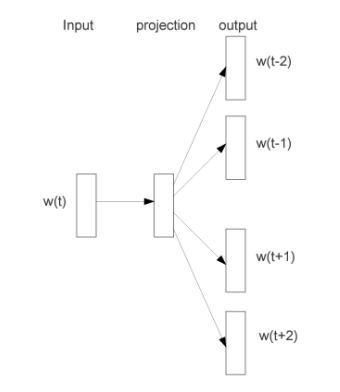
\includegraphics[width=\linewidth, height = 85mm]{img5}
    \caption{\small \centering Illustration of how Word2vec 
    technology works. \label{figure5}}
\end{figure}

\par Following the Word2vec principle, we can build a
semantic model to determine the semantic image of an
image. Thus, the image is converted into a covariance
ratio vector, where each cell uniquely defines the covariance of the two spectral layers. Consequently, if defining
vectors are selected for each class, then by the difference
between the vectors of the vector space, the dimension
of which is n*n, where n is the number of spectral bands
in the image, it will be possible to predict which class
the image belongs to by the semantic difference of the
vectors. 
\par Using this semantic approach, we convert the image
into a covariance ratio vector. Each element in this vector
encapsulates the covariance between the two spectral
layers, encoding not only spectral information but also
semantic nuances. By selecting definition vectors for each
terrain category, we create a semantic reference frame.
Subsequently, using the semantic differences between
these vectors within a vector space (which is expanded
according to the number of spectral bands in the image), 
images can be accurately classified based on their
semantic properties. By leveraging semantic techniques,
we overcome the limitations of traditional pixel-based
analysis and gain a deeper understanding of the semantic
landscape of multispectral images. 

\begin{center}
    \uppercase\expandafter{\romannumeral 6}. Demonstration of the method 
\end{center}

\par To demonstrate how the method works, consider matrices for 
three different classes: Industrial, Forest, SeaLake. All 
three classes have different spectral characteristics that 
will uniquely determine the covariance matrix for the images 
representing the class. By calculating the average value of 
the covariance matrix for classes whose sample included 1000 
images, as well as the vector of eigenvalues of these matrices.
\vspace{10pt}

\noindent \textit{A. Calculation of class matrices} 
\vspace{5pt} 

\par Matrix for class Industrial: 
\par [[1 0.981 0.971 0.839 0.328 0.33 0.583 0.676] 
\par [0.981 1. 0.976 0.876 0.414 0.426 0.64 0.696] 
\par [0.971 0.976 1. 0.877 0.347 0.348 0.653 0.738]
\par [0.839 0.876 0.877 1. 0.549 0.45 0.823 0.823]
\par [0.328 0.414 0.347 0.549 1. 0.886 0.59 0.323]
\par [0.33 0.426 0.348 0.45 0.886 1. 0.504 0.255] 
\par [0.583 0.64 0.653 0.823 0.59 0.504 1. 0.903] 
\par [0.676 0.696 0.738 0.823 0.323 0.255 0.903 1. ]] 
\vspace{10pt}

\noindent Eigenvalues: 
\par [5.566 1.449 0.706 0.145 0.059 0.012 0.024 0.041] 
\vspace{10pt}

\noindent Matrix for class Forest: 
\par [[1. 0.878 0.907 0.853 0.724 0.75 0.841 0.854] 
\par [0.878 1. 0.907 0.888 0.805 0.856 0.861 0.863] 
\par [0.907 0.907 1. 0.917 0.738 0.731 0.882 0.907] 
\par [0.853 0.888 0.917 1. 0.888 0.793 0.972 0.976] 
\par [0.724 0.805 0.738 0.888 1. 0.898 0.901 0.857] 
\par [0.75 0.856 0.731 0.793 0.898 1. 0.794 0.755] 
\par [0.841 0.861 0.882 0.972 0.901 0.794 1. 0.992] 
\par [0.854 0.863 0.907 0.976 0.857 0.755 0.992 1. ]] 
\vspace{10pt}

\noindent Eigenvalues: 
\par [5.568 1.259 0.627 0.218 0.015 0.066 0.136 0.112] 
\vspace{10pt}

\noindent Matrix for class SeaLake: 
\par [[1. 0.492 0.446 0.366 0.27 0.23 0.295 0.289]
\par [0.492 1. 0.477 0.408 0.32 0.26 0.329 0.296] 
\par [0.446 0.477 1. 0.532 0.418 0.394 0.402 0.373] 
\par [0.366 0.408 0.532 1. 0.583 0.552 0.537 0.501] 
\par [0.27 0.32 0.418 0.583 1. 0.582 0.585 0.519]
\par [0.23 0.26 0.394 0.552 0.582 1. 0.54 0.482] 
\par [0.295 0.329 0.402 0.537 0.585 0.54 1. 0.561] 
\par [0.289 0.296 0.373 0.501 0.519 0.482 0.561 1. ]] 
\vspace{10pt}

\noindent Eigenvalues: 
\par [4.047 1.147 0.589 0.506 0.492 0.383 0.413 0.425] 
\vspace{20pt}

\par And also consider two images from the dataset,
Industrial-1011, shown in Figure 2, and SeaLake-1016,
shown in Figure \ref{figure6}.

\begin{figure}[H]
    \centering
    
\includegraphics[width=0.5\linewidth]{img6}
    \caption{\small \centering SeaLake-1016 in RGB spectral bands. \label{figure6}}
\end{figure} 

\noindent \textit{B. Calculation of image matrices} 
\vspace{5pt}

\par The first proposed method for determining the class
of an image will be the difference in the metrics of the
matrix space L0. This method allows you to quickly and
even visually determine whether an image belongs to a
class. The main problem of this method is reducing the
dimension of space from eight stripes to one number,
as a result of which collisions arise when semantically
different vectors return a measure that is close in value.
Because of this, a significant number of errors arise when
determining the class of an image. 
\par The second method for determining the class membership of an image is the nearest neighbor search algorithm.
This algorithm consists of three steps: \vspace{-8pt}

\begin{enumerate}[label=\arabic*)]
    \item  The distance between each image and the eigenvectors of each class is calculated. The distance is
    taken to be the quadratic difference of vectors.\vspace{-6pt}
    \item Find the minimum distance for each image.\vspace{-6pt}
    \item The class to which the image belongs is determined
    by comparing the minimum distances.\vspace{-6pt}
\end{enumerate}

\par This method requires a little more calculations, but
it takes into account the ratio of the spectral bands of
the matrices in a certain order, as well as the difference
between the corresponding bands. 

\par The image Industrial-1011 obtained the following
values of the covariance matrices and eigenvectors: 
\vspace{10pt}

\noindent Matrix for class Industrial-1011: 
\par [[1. 0.982 0.957 0.841 0.136 0.195 0.564 0.774]
\par [0.982 1. 0.975 0.873 0.214 0.275 0.604 0.778]
\par [0.957 0.975 1. 0.899 0.18 0.216 0.63 0.818] 
\par [0.841 0.873 0.899 1. 0.383 0.321 0.816 0.929]
\par [0.136 0.214 0.18 0.383 1. 0.925 0.69 0.36 ] 
\par [0.195 0.275 0.216 0.321 0.925 1. 0.608 0.302]
\par [0.564 0.604 0.63 0.816 0.69 0.608 1. 0.894] 
\par [0.774 0.778 0.818 0.929 0.36 0.302 0.894 1. ]] 
\vspace{10pt}

\noindent Eigenvalues: 
\par [5.47 1.862 0.487 0.089 0.042 0.032 0.006 0.014] 
\vspace{10pt}

\noindent Based on the calculation results, image Industrial1011, the quadratic distance between the image vector
and the Industrial class vector is 0.482, the Forest class
vector is 0.662, and the SeaLake class vector is 1.839.
For clarity, distances are rounded to the third decimal
place. The probability of an image belonging to the
Industrial class is 84\%, to the Forest class is 78\%, and
to the SeaLake class is 38\%. Thus, we can conclude that
the image belongs to the Industrial class, but it is worth
noting the presence of local vegetation in the image. 

\par The SeaLake-1016 image obtained the following
values of covariance matrices and matrix space norms: 
\vspace{10pt}

\noindent Matrix for class SeaLake-1016 : 
\par [[1. 0.465 0.383 0.433 0.409 0.306 0.316 0.124]
\par [0.465 1. 0.56 0.621 0.605 0.459 0.477 0.137] 
\par [0.383 0.56 1. 0.546 0.512 0.439 0.386 0.172] 
\par [0.433 0.621 0.546 1. 0.647 0.51 0.481 0.202] 
\par [0.409 0.605 0.512 0.647 1. 0.553 0.562 0.238]
\par [0.306 0.459 0.439 0.51 0.553 1. 0.42 0.174] 
\par [0.316 0.477 0.386 0.481 0.562 0.42 1. 0.095] 
\par [0.124 0.137 0.172 0.202 0.238 0.174 0.095 1. ]] 
\vspace{10pt}

\noindent Eigenvalues: 
\par [3.981 0.955 0.746 0.611 0.553 0.453 0.371 0.331] 
\vspace{10pt}

\noindent Based on the calculation results, image Industrial1011, the quadratic distance between the image vector
and the Industrial class vector is 1.902, the Forest
class vector is 1.823, and the SeaLake class vector is
0.310. For clarity, distances are rounded to the third
decimal place. The probability of an image belonging
to the Industrial class is 47\%, to the Forest class is
49\%, and to the SeaLake class is 92\%. Thus, we can
conclude that the image belongs to the SeaLake class,
and unambiguously. 

\begin{center}
    Diagram of the algorithm 
\end{center} 
\vspace{-5pt}
\par The general diagram of the algorithm is presented in Figure 
\ref{figure7}. 

\begin{figure}[H]
    \centering
    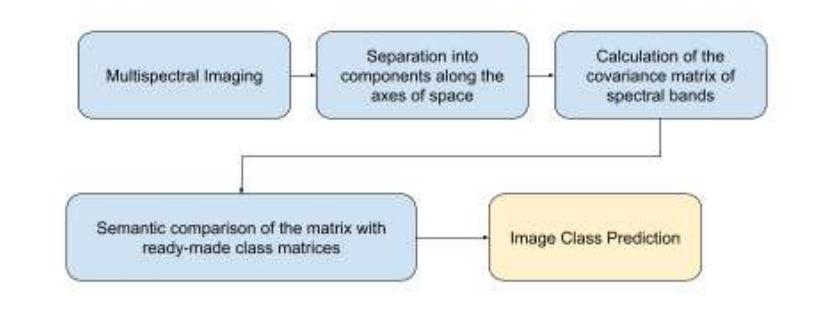
\includegraphics[width=\linewidth]{img7}
    \caption{\small \centering General diagram of the algorithm. \label{figure7}}
    
\end{figure} 

\begin{center}
    Acknowledgment \par
\end{center} 

Financial support for the project “Agreement on the
development of technology for developing algorithms
for processing images of remote sensing of the Earth”,
agreement number: 22CETC19-ICN1785. \par

\newcolumn

\fontsize{8pt}{10pt}\selectfont
\begin{thebibliography}{10}
    \bibitem{} J. Shotton, J.M. Winn, C. Rother, A. Criminisi, “TextonBoost:
    Joint Appearance, Shape and Context Modeling for Multi-class
    Object Recognition and Segmentation,” A. Leonardis, H. Bischof,
    A. Pinz, ECCV 2006, Part I. LNCS, vol. 3951, pp. 1–15. Springer,
    Heidelberg, 2006. \vspace{-7pt}
    \bibitem{} G. Csurka, F. Perronnin, “An efficient approach to semantic
    segmentation,” IJCV 95, 2011. \vspace{-7pt}
    \bibitem{} J. Verbeek, B. Triggs, “Region classification with markov field
    aspects models,” CVPR, 2007. \vspace{-7pt}
    \bibitem{} L. Ladicky, C. Russell, P. Kohli, P.H.S. Torr, “Graph Cut Based
    Inference with Co-occurrence Statistics,” K. Daniilidis, P. Mara-
    gos, N. Paragios: ECCV 2010, Part V. LNCS, vol. 6315, pp.
    239–253. Springer, Heidelberg, 2010.\vspace{-7pt}
    \bibitem{} G.D. Finlayson, M.S. Drew, B.V. Funt, “Color constancy: gener-
    alized diagonal transforms suffice,” Journal of the Optical Society
    of America 11, 3011–3019, 1994. \vspace{-7pt}
    \bibitem{} G. Eason, B. Noble, and I. N. Sneddon, “On certain integrals
    of Lipschitz-Hankel type involving products of Bessel functions,”
    Phil. Trans. Roy. Soc. London, vol. A247, pp. 529–551, April
    1955. \vspace{-7pt}
    \bibitem{} Patrick Helber, Benjamin Bischke, Andreas Dengel, Damian
    Borth. “Eurosat: a new dataset and deep learning benchmark for
    land use and land cover classification.” IEEE Journal on Selected
    Topics in Applied Earth Observation and Remote Sensing, 2019. \vspace{-7pt}
    \bibitem{} Patrick Helber, Benjamin Bischke, Andreas Dengel. “Introducing
    EuroSAT: a new dataset and deep learning benchmark for land
    use and land cover classification.” 2018 IEEE International Sym-
    posium on Geosciences and Remote Sensing. \vspace{-7pt}
    \bibitem{} Santosh Kumar R., “Principal Component Analysis: Drilling
    Insight through Image Visualization,” 2020. \vspace{-7pt}
    \bibitem{} Mikolov T., Chen K., Corrado G., Dean J. Efficient Estimation
    of Word Representations in Vector Space. In Proceedings of
    Workshop at ICLR, 2013.
\end{thebibliography}

\vspace{+10pt}
\normalsize

\begin{center}
    \textbf{\fontsize{12pt}{16pt}\selectfont ОПРЕДЕЛЕНИЕ КЛАССА 
    МУЛЬТИСПЕКТРАЛЬНОГО
    ИЗОБРАЖЕНИЯ ПО
    СЕМАНТИЧЕСКОЙ РАЗНОСТИ
    КОВАРИАЦИОННЫХ МАТРИЦ}
\end{center}

\noindent\large Бу Цин, Недзьведь А. А., Белоцерковский А.
\vspace{0pt}


\par Аннотация: В данной статье проведено исследование 
спутниковых мультиспектральных изображений,
спектральных данных местности, а также представлен
метод определения принадлежности изображений к
классам местности с использованием семантического
анализа вектора собственных значений ковариационной 
матрицы спутникового мультиспектрального изображения.

\begin{flushright}
    Received 27.03.2024
\end{flushright}

\end{multicols*}
\end{document}  
